%%%%%%%%%%%%%%%%%%%%%%%%%%%%%%%%%%%%%%%%%
% Vertical Line Title Page
% LaTeX Template
% Version 2.0 (22/7/17)
%
% This template was downloaded from:
% http://www.LaTeXTemplates.com
%
% Original author:
% Peter Wilson (herries.press@earthlink.net) with modifications by:
% Vel (vel@latextemplates.com)
%
% License:
% CC BY-NC-SA 3.0 (http://creativecommons.org/licenses/by-nc-sa/3.0/)


\documentclass[a4paper, 11pt]{book} % A4 paper size and default 11pt font size
\usepackage[utf8]{inputenc} % Required for inputting international characters
\usepackage[T1]{fontenc} % Output font encoding for international characters
\usepackage{stix} % Use the STIX fonts
\usepackage{graphicx}
\usepackage{mathtools}
\usepackage{setspace}

%code to adjust margins
\addtolength{\oddsidemargin}{-.875in}
	\addtolength{\evensidemargin}{-.875in}
	\addtolength{\textwidth}{1.75in}

	\addtolength{\topmargin}{-.875in}
	\addtolength{\textheight}{1.75in}

\makeatletter

\begin{document}

%----------------------------------------------------------------------------------------
%	TITLE PAGE
%----------------------------------------------------------------------------------------

\begin{titlepage} % Suppresses displaying the page number on the title page and the subsequent page counts as page 1
	
	\raggedleft % Right align the title page
	
	\rule{1pt}{\textheight} % Vertical line
	\hspace{0.05\textwidth} % Whitespace between the vertical line and title page text
	\parbox[b]{0.75\textwidth}
	{ % Paragraph box for holding the title page text, adjust the width to move the title page left or right on the page
		
		{\Huge\bfseries MATH 310  \\[0.5\baselineskip] Probability \& Statistics}\\[2\baselineskip] % Title
		{\large\textit{Project Observations}}\\[4\baselineskip] % Subtitle or further description
		{\Large\textsc{muhammad munawwar anwar (ma04289) \\ khubaib naeem kasbati (kk04333) }} % Author name, lower case for consistent small caps 
		 % Author name, lower case for consistent small caps
		
        {\large June 19, 2020}\\[2cm] % Date, change the \today to a set date if you want to be precise
		\vspace{0.5\textheight} % Whitespace between the title block and the publisher

		{\noindent Habib University}\\[\baselineskip] % Publisher and logo
		
	}
	
    
\end{titlepage}
%----------------------------------------------------------------------------------------
\tableofcontents




\newpage

\addcontentsline{toc}{chapter}{Tasks}
\section*{Tasks}


\addcontentsline{toc}{subsection}{Task 1}
\subsection*{Task 1}

In task 1 when we the ran the simulation 10000 times, where each simulation consisted of 50 steps and the probability for the walk to move left, right or stay equally likely and the starting position was the point zero,  the expected value of the distance travelled was 49.9875.The resulting distrubution can be found in Figure \ref{fig:mesh1}.
Furethermore, the distrubution was symmetric about the mean value. However, if the chosen starting point is not zero or the probability to move left, right or stay is unequal then the mean of the distrubution shifts or it becomes left or right skewed.

\addcontentsline{toc}{subsection}{Task 2}
\subsection*{Task 2}

In task 2 when we the ran the simulation 10000 times, where in each simulation the starting distance x between two people was  50 and the probability for the both person to move left, right or stay was equally likely and same, the expected value of time required for both people to meet was \(8468.63\) . The distribution can be seen in Figure \ref{fig:mesh2}
The distrubution is left skewed. The starting distance x between the two people has linear relation with number of time required to meet. \\
Our model is based on the assumption that 


\addcontentsline{toc}{subsection}{Task 3}
\subsection*{Task 3}

Suppose that a walker is at the position $P = (P_1,P_2)$ inside the test region at $(k-1)^{th}$ step, but
the next step would be to a position $ Q = (Q_1,Q_2) $ that is either on the boundary or beyond the 
boundary. We divide the contemplated step from P to Q into two steps  : (1) an
actual step (the $k^{th}$) to the boundary point $P^{\prime}$,where the segment $\vec{PQ} $ intersects the boundary,  and then (2)
a step $(k+1)^{st}$ of one unit to a point $Q^{\prime}$ inside the circle. Specifically, let $P^{\prime}$ be the
point where the walker hits or would cross the boundary and $\alpha$ the angle of incidence of the walker's path
with the tangent line to the circle at  $P^{\prime}$. The walker takes a step (kth step) to $P^{\prime}$ and then takes a step((k+1)st) back into the 
circle on a path which forms an angle $\alpha$ with the tangent line at $P^{\prime}$. This Reflection method can be seen in Figure \ref{fig:mesh3}







\addcontentsline{toc}{subsection}{Task 4}
\subsection*{Task 4}

In task 1 when we the ran the simulation 10000 times, where each simulation consisted of 50 steps and the step was modeled as a uniform random variable between 0 and 1 , the expected value of the distance travelled was 25.0.
Furethermore, the distrubution was symmetric about the mean value. However, if the chosen starting point is not zero or the probability to move left, right or stay is unequal then the mean of the distrubution shifts or it becomes left or right skewed. The distribution can be seen in Figure \ref{fig:mesh4}.


25.03133906218428


\addcontentsline{toc}{subsection}{Task 5}
\subsection*{Task 5}

\addcontentsline{toc}{subsection}{Task 6}
\subsection*{Task 6}


\addcontentsline{toc}{subsection}{Task 7}
\subsection*{Task 7}

\addcontentsline{toc}{subsection}{Task 8}
\subsection*{Task 8}



\cleardoublepage

\addcontentsline{toc}{chapter}{Figures}
% \listoffigures
\section*{Figures}
\begin{figure}[h]
	\centering
	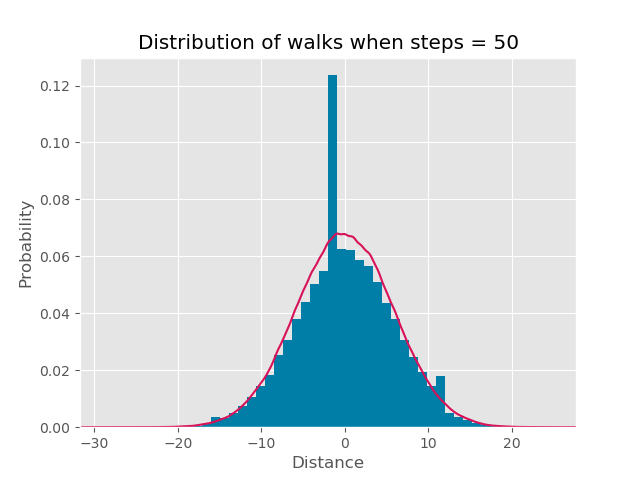
\includegraphics[width=0.7\textwidth]{Task 1.png}
	\caption{One Dimensional Discrete Random Walk}
	\label{fig:mesh1}
\end{figure}

\begin{figure}[h]
	\centering
	\includegraphics[width=0.7\textwidth]{task 2.png}
	\caption{Distrubution of time required for two people who are intially 50 units away}
	\label{fig:mesh2}
\end{figure}
\begin{figure}[h]
	\centering
	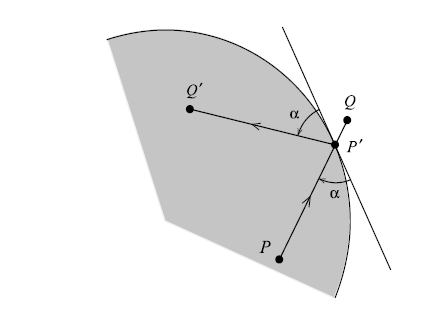
\includegraphics[width=0.8\textwidth]{ReflectionRule.png}
	\caption{Reflection from the Circumference}
	\label{fig:mesh3}
\end{figure}

\begin{figure}[h]
	\centering
	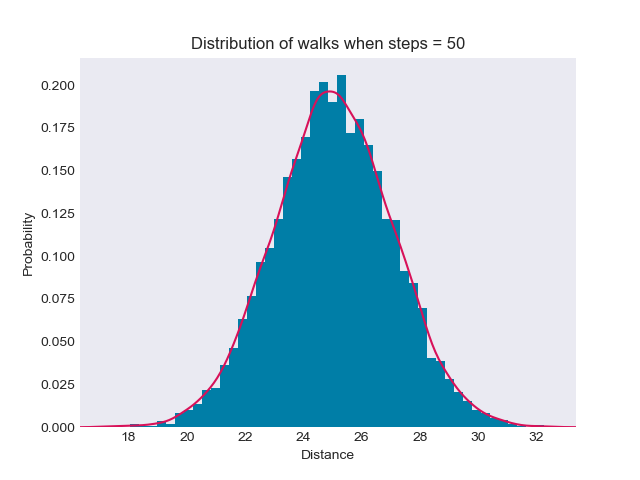
\includegraphics[width=0.8\textwidth]{task 4.png}
	\caption{One Dimensional Discrete Random Walk}
	\label{fig:mesh4}
\end{figure}



\newpage
\addcontentsline{toc}{chapter}{Bibliography}
\begin{thebibliography}{9}
	% \bibitem{SeabornPydata} 
	% Seaborn: Pydata : Official Seaborn Tutorial : Aesthetics,
	% \\\texttt{https://seaborn.pydata.org/tutorial/aesthetics.html}
	
	% \bibitem{stackexchange} 
	% Stack Exchange: Tex : Is there a command to write the form of a combination or permutation?,
	% \\\texttt{https://tex.stackexchange.com/questions/107125/is-there-a-command-to-write-\\the-form-of-a-combination-or-permutation}
	
	% \bibitem{stackexchange1} 
	% Stack Exchange: Tex : Superscript outside math mode,
	% \\\texttt{https://tex.stackexchange.com/questions/47324/superscript-outside-math-mode}
	
	% \bibitem{stackexchange2} 
	% Stack Exchange: Tex : How can I use BibTeX to cite a web page?,
	% \\\texttt{https://tex.stackexchange.com/questions/3587/how-can-i-use-bibtex-to-cite-a-\\web-page}
	
	% \bibitem{rectitations} 
	% Recitations And Lecture Notes
	
\end{thebibliography}
  


\end{document}
